%%%
 %
 % Copyright (C) 2019 Ángel Iván Gladín García
 %
 % This program is free software: you can redistribute it and/or modify
 % it under the terms of the GNU General Public License as published by
 % the Free Software Foundation, either version 3 of the License, or
 % (at your option) any later version.
 %
 % This program is distributed in the hope that it will be useful,
 % but WITHOUT ANY WARRANTY; without even the implied warranty of
 % MERCHANTABILITY or FITNESS FOR A PARTICULAR PURPOSE.  See the
 % GNU General Public License for more details.
 %
 % You should have received a copy of the GNU General Public License
 % along with this program.  If not, see <http://www.gnu.org/licenses/>.
%%%

%%%%%%%%%%%%%%%%%%%%%%%%%%%%%%%%%%%%%%%%%%%%%%%%%%%%%%%%%%%%%%%%%%%%%%%%%%%%%%%%%%%%%%%%%
\documentclass[12pt,letterpaper]{article}
\usepackage[margin=.6in]{geometry}
\usepackage[utf8]{inputenc}
\usepackage[spanish]{babel}
\decimalpoint

\usepackage{listings}
\usepackage{color}
\usepackage{graphicx}
\usepackage{enumerate}
\usepackage{enumitem}
\usepackage{float}

\usepackage{longtable}
\usepackage{hyperref}
\usepackage{commath}

\usepackage{bbm}
\usepackage{dsfont}
\usepackage{mathrsfs}
\usepackage{amsmath,amsthm,amssymb}
\usepackage{mathtools}
\usepackage{longtable}

%%%%%%%%%%%%%%%%%%%%%%%%%%%%%%%%%%%%%%%%%%%%%%%%%%%%%%%%%%%%%%%%%%%%%%%%%%%%%%%%%%%%%%%%%%%%%%%%5

\usepackage{import}

\usepackage[utf8]{inputenc}

\usepackage{listings}
\usepackage{color}

\definecolor{codegreen}{rgb}{0,0.6,0}
\definecolor{codegray}{rgb}{0.5,0.5,0.5}
\definecolor{codepurple}{rgb}{0.58,0,0.82}
\definecolor{backcolour}{rgb}{0.95,0.95,0.92}

\lstdefinestyle{mystyle}{
    backgroundcolor=\color{backcolour},   
    commentstyle=\color{codegreen},
    keywordstyle=\color{magenta},
    numberstyle=\tiny\color{codegray},
    stringstyle=\color{codepurple},
    basicstyle=\footnotesize,
    breakatwhitespace=false,         
    breaklines=true,                 
    captionpos=b,                    
    keepspaces=true,                 
    numbers=left,                    
    numbersep=5pt,                  
    showspaces=false,                
    showstringspaces=false,
    showtabs=false,                  
    tabsize=2
}
\usepackage[autostyle]{csquotes}

\lstset{style=mystyle}
%%%%%%%%%%%%%%%%%%%%%%%%%%%%%%%%%%%%%%%%%%%%%%%%%%%%%%%%%%%%%%%%%%%%%%%%%%%%%%%%%%%%%%%%%


%%%%%%%%%%%%%%%%%%%%%%%%%%%%%%%%%%%%%%%%%%%%%%%%%%%%%%%%%%%%%%%%%%%%%%%%%%%%%%%%%%%%%%%%%
\newcommand{\Z}{\mathbb{Z}}
\newcommand{\N}{\mathbb{N}}
\newcommand{\Q}{\mathbb{Q}}
\newcommand{\R}{\mathbb{R}}
\newcommand{\Pro}{\mathds{P}}
\newcommand{\Oh}{\mathcal{O}} %% Notacion "O"
\newcommand{\lra}{\longrightarrow}
\newcommand{\ra}{\rightarrow}
\newcommand{\ord}{\text{ord}}
\newcommand{\sol}{\textbf{\underline{Solución}: }} %% Solucion
\newcommand{\af}{\textbf{\underline{Afirmación}: }}
\newcommand{\cej}{\textbf{\underline{Contraejemplo}: }}

%%%%%%%%%%%%%%%%%%%%%%%%%%%%%%%%%%%%%%%%%%%%%%%%%%%%%%%%%%%%%%%%%%%%%%%%%%%%%%%%%%%%%%%%%

\begin{document}

%%%%%%%%%%%%%%%%%%%%%%%%%%%%%%%%%%%%%%%%%%%%%%%%%%%%%%%%%%%%%%%%%%%%%%%%%%%%%%%%%%%%%%%%%
\title{
        Universidad Nacional Autónoma de México\\
        Facultad de Ciencias\\
        Complejidad Computacional\\
    \vspace{1cm}
    \large
        \textbf{Tarea}\\
        \textbf{\textit{Problema de asignación óptima de salones resuelto con Búsqueda Tabú}}
}
\author{
    Ángel Iván Gladín García\\
    No. cuenta: 313112470\\
    \texttt{angelgladin@ciencias.unam.mx}
}
\date{4 de diciembre 2019}
\maketitle
%%%%%%%%%%%%%%%%%%%%%%%%%%%%%%%%%%%%%%%%%%%%%%%%%%%%%%%%%%%%%%%%%%%%%%%%%%%%%%%%%%%%%%%%%

%%%%%%%%%%%%%%%%%%%%%%%%%%%%%%%%%%%%%%%%%%%%%%%%%%%%%%%%%%%%%%%%%%%%%%%%%%%%%%%%%%%%%%%%%
\newtheorem{theorem}{Teorema}
\newtheorem{example}{Ejemplo}
\newtheorem{corollary}{Corolario}
\newtheorem{lemma}{Lemma}
\newtheorem{definition}{Definicion}
\newtheorem{prop}{Proposicion}
%%%%%%%%%%%%%%%%%%%%%%%%%%%%%%%%%%%%%%%%%%%%%%%%%%%%%%%%%%%%%%%%%%%%%%%%%%%%%%%%%%%%%%%%%

%%%%%%%%%%%%%%%%%%%%%%%%%%%%%%%%%%%%%%%%%%%%%%%%%%%%%%%%%%%%%%%%%%%%%%%%%%%%%%%%%%%%%%%%%
\section{Descripción del problema}
El artículo habla sobre el problema de la asignación de salones como un problema de optimización matemática.

Al inicio de cada periodo académico la administación conoce las asignaturas a las que los estudiantes
van a a ir, y también deben de distribuirlas en su planta física de tal forma que todos los interesados
reciban las materias que pidieron. Pero el modelo tiene un conjunto de restricciones llamadas
\textbf{duras} (su cumplimiento es obligatorio) y \textbf{blandas} (su cumplimiento es optativo).
Si las restricciones anteriores son satisfechas de dice que la propuesta dada es \textbf{factible}. 
El tipo de restricción llamada \text{blanda} dice que su cumplimiento no es obligatorio
pero miden el grado de satifacción de los estudiante.

Este problema combinatorio es clasificado como del tipo no lineal entero mixto y es de difícil solución.
Clasificado como NP completo

Se han descrito varios métodos para resolver este problema, tales como: métodos secuenciales, 
métodos de clusterización, métodos basados en restricciones, y los métodos metaheuríticos.

Se aborda este problema para la solución del problema de asignación óptima de salones usando la
técnica de \textbf{Búsqueda Tabú}.

Se va a plantear algoritmos constructivos para generar una configuración incial de calidad y también
se va a definir la estructura de vecindad para la búsqueda local con \textit{Búsqueda Tabú}.

\section{Planteamiento del problema}
La naturaleza de este tipo de problemas son de organizar una secuencia de eventos, en un periodo de tiempo
determinado satisafacionedo un conjunto de restricciones. En este caso como es la asignaciónde de salones
las restricciones son; asignación de recursos, asignación de tiempo, restricciones de tiempo entre sesiones,
dispersión de las sesiones, coherencia de las reuniones, capacidad de las salas, continuidad.

En este artículo como ya se mencionó antes, se busca el cumplimientos de restricciones duras y las restricciones
blandas (que nos son obligatorias que se cumplan).

La restricciones duras en este caso son; que el salón asignado cumpla con los requisitos apropiados para el evento
que se hará, los horarios (que no haya conflictos), y que un salón no tenga dos eventos a la misma hora.

Si todos esas restricciones de complen se dice que la propuesta es \textbf{factible} pero como queremos
que los estudiantes hagan su actividades de forma cómoda, así que queremos que se cumpla el mayor número de
restricciones blandas. Si una restricción blanda no se cumple será penalizada en \textbf{la función objetivo}
incrementando su valor en 1 por cada restricción violada,

Analizando todo eso, se empiza a formalizar el problema de programación de horarios de clase, de tal forma que si
se cumplen las restricciones duras, se \textbf{minimizan} las restricciones blandas.

\section{Búsqueda Tabú}
\blockquote{
La \textit{Búsqueda Tabú} es una técnica de optimización combinatorial que proviene de la inteligencia
artificial y usa conceptos de memoria adaptativa y exploración sensible.
Un algoritmo de Búsqueda Tabú completo utiliza técnicas de exploración y de memoria avanzadas, como son:
memoria de corto y largo plazo, estrategias de intensificación, diversificación, oscilación estratégica,
\textit{path relinking} y lista de configuraciones de élite, entre otras.
}
\subsection{Función objetivo}
\[
    \min f(x) \qquad x \in X
\]
Donde $f$ es una función y $X$ es un conjunto de restricciones.

\section{Modelado matemático y codificación}
La información del problema se maneja por medio de vectores y matrices en los cuales se indica:
\begin{itemize}
    \item Matriz de booleanos que indica si un evento (fila) requiere cierta característica (columna).
    \item Matriz de booleanos que indica si un salón (fila) requiere cierta característica.
    \item Un vector que indica la capacidad del salón $i$.
    \item Matriz de booleanos que indica que indica si un estudiante está matriculado en un evento.
    \item Matriz de booleanos que indica que indica los eventos de los salones, indicando si el evento
    $i$ se puede programar en el evento $j$.
\end{itemize}

Lo que se busca minimizar es:
$$z = hf + hu + hc$$
Donde la variable $hf$ representa el número de eventos programadas al final de cada día para todos
los estudiantes, $hu$ el número de eventos únicos en cada día para todos los estudiantes, y
$hc$ representa los casos en que se programan más de dos eventos consecutivos en un día para todos los estudiantes.

\section{Aplicación de Búsqueda Tabú a la programación óptima de horarios de clase}
Tendrá cuatro fases para la solución de problema.
\begin{enumerate}
    \item Tener una programación inicial para que los eventos sean programados con pocas restricciones
    duras violadas.
    \item Búsqueda local para disminuir restricciones duras violadas.
    \item Alcancar una solución factible, en la que se cumplen las restricciones duras usando
    la \textbf{Búsqueda Tabú} para minimizar restricciones duras.
    \item Usar \textbf{Búsqueda Tabú} para minimizar restricciones blandas, manteniendo la
    factibilidad de la configuración.
\end{enumerate}
\subsection{Generación de configuración inicial}
Se hace de forma prioritaria teniendo los eventos que tiene menor número de salones habilitados.
Esto se hace ordenando los eventos de menor a mayor número de salones habilitados. Al principio
de programan los eventos que solo se pueden hacer en un salón en específico. Se van
\textit{emperajendo} así salones con los eventos de forma creciente.

Se puede ver en este diagrama la forma de hacerse:
\begin{figure}[H]
	\centering
		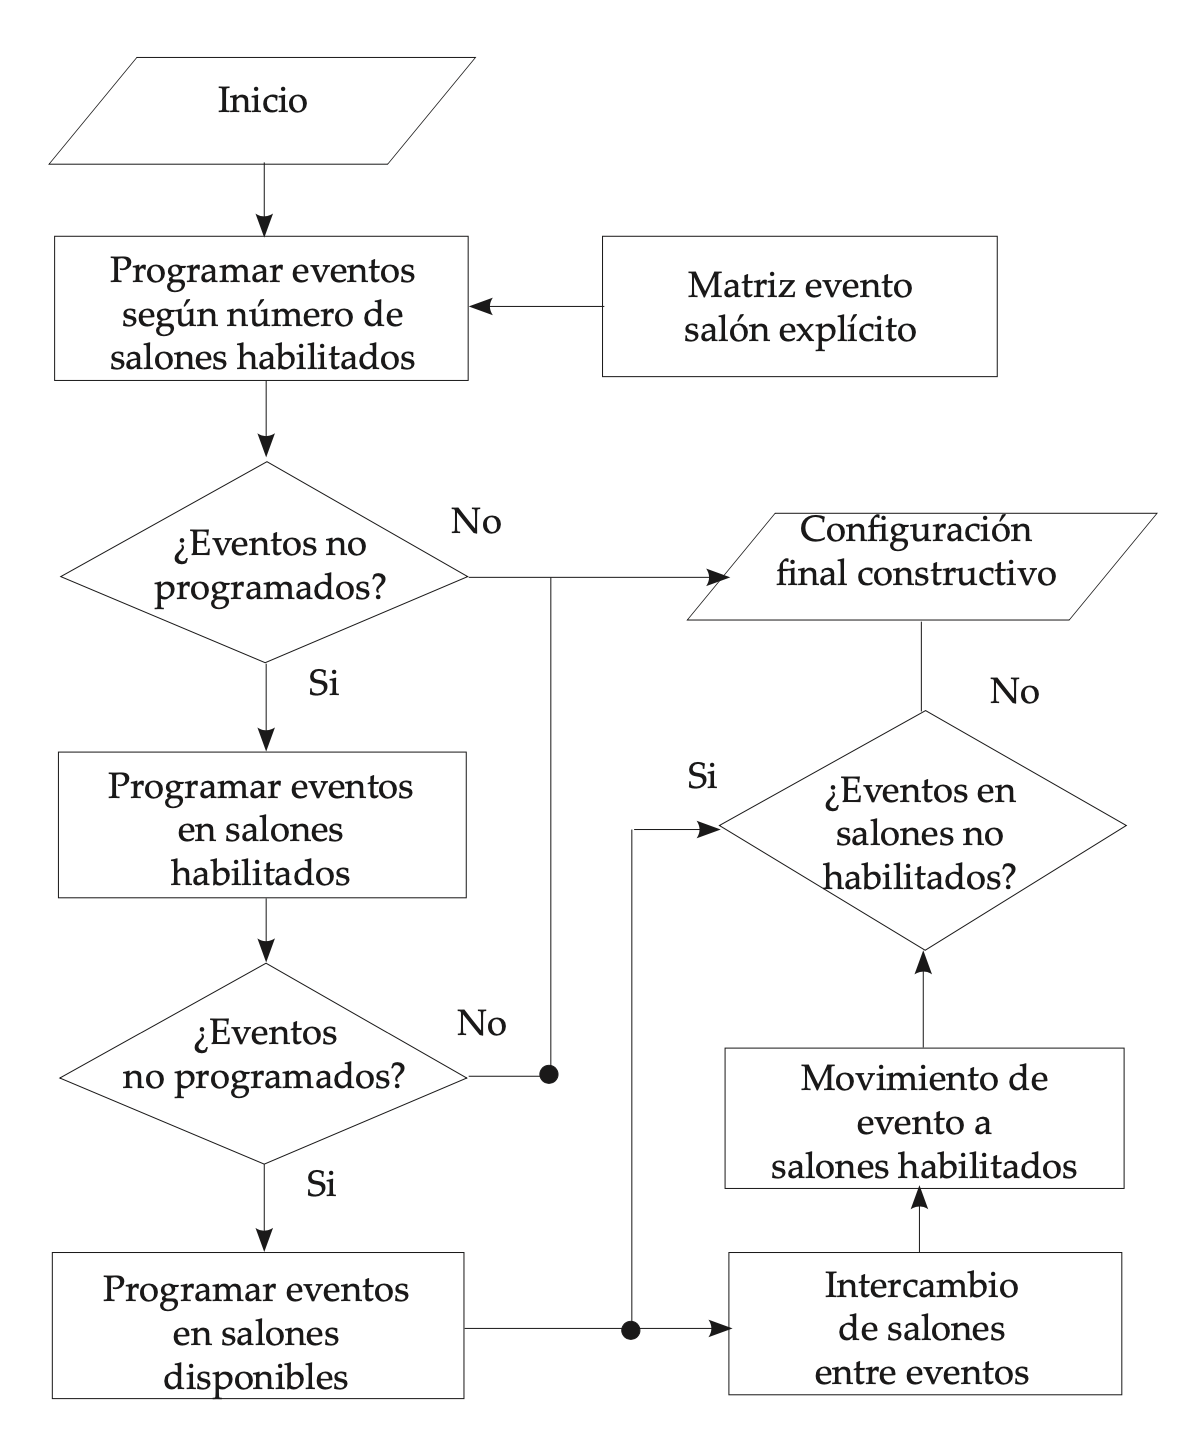
\includegraphics[scale=0.4]{assets/1.png}
\end{figure}

\subsection{Evaluación de la función objetivo}
Lo que se hace es contar el número de restricciones duras y blandas que son violadas.
Se revisa las restricciones duras de la configuración, checando si el salón en el que se hará
el evento este habilitado, ósea que tiene las capacidades y características que se necesitan.
Después de checa si hay crece en los horarios para los estudiantes, se hace esto checando
las combinaciones de de dos salones a la misma hota.

\subsection{Índice de sensibilidad}
Se crea un índice para cada evento, usando un contador que tiene el número de problemas asociados
a este. Esto sirve para el proceso de búsqueda.

\subsection{Estructura de vecindad}
El vecindario de una configuración consiste en configuraciones obtenidas haciendo pequeños cambios a
la configuración actual. Un pequeño cambio en la configuración puede ser la modificación de hora o de
salón para un evento. Con el fin de alterar la hora de un evento, sin que se afecte su fac- tibilidad
por el salón, se puede intercambiar el bloque de tiempo de dicho evento con el de otro suceso en el mismo lugar.

Se generan configuraciones vecinas a partitr de un intercambio del bloque de tiempo del evento con otro suceso en el
mismo salón y un ovimiento del evento a un bloque de tiempo libre, en un salón habilitado para la actividad.

\subsection{Manejo de la memoria de corto plazo}
En Búsqueda Tabú se utiliza una estructura de memoria de corto plazo que evita regresar a configuraciones
ya visitadas, con lo que se puede escapar de óptimos locales en el proceso de búsqueda.

\subsection{Criterio de aspiración}
\blockquote{
Si se da el caso en que la mejor configuración vecina se encuentre prohibida, y su función objetivo mejora la mejor función
objetivo encontrada hasta el momento en la búsqueda (valor de la incumbente), el criterio de aspiración permite seleccionar
esta configuración a pesar de estar excluída.
}

\begin{figure}[H]
	\centering
		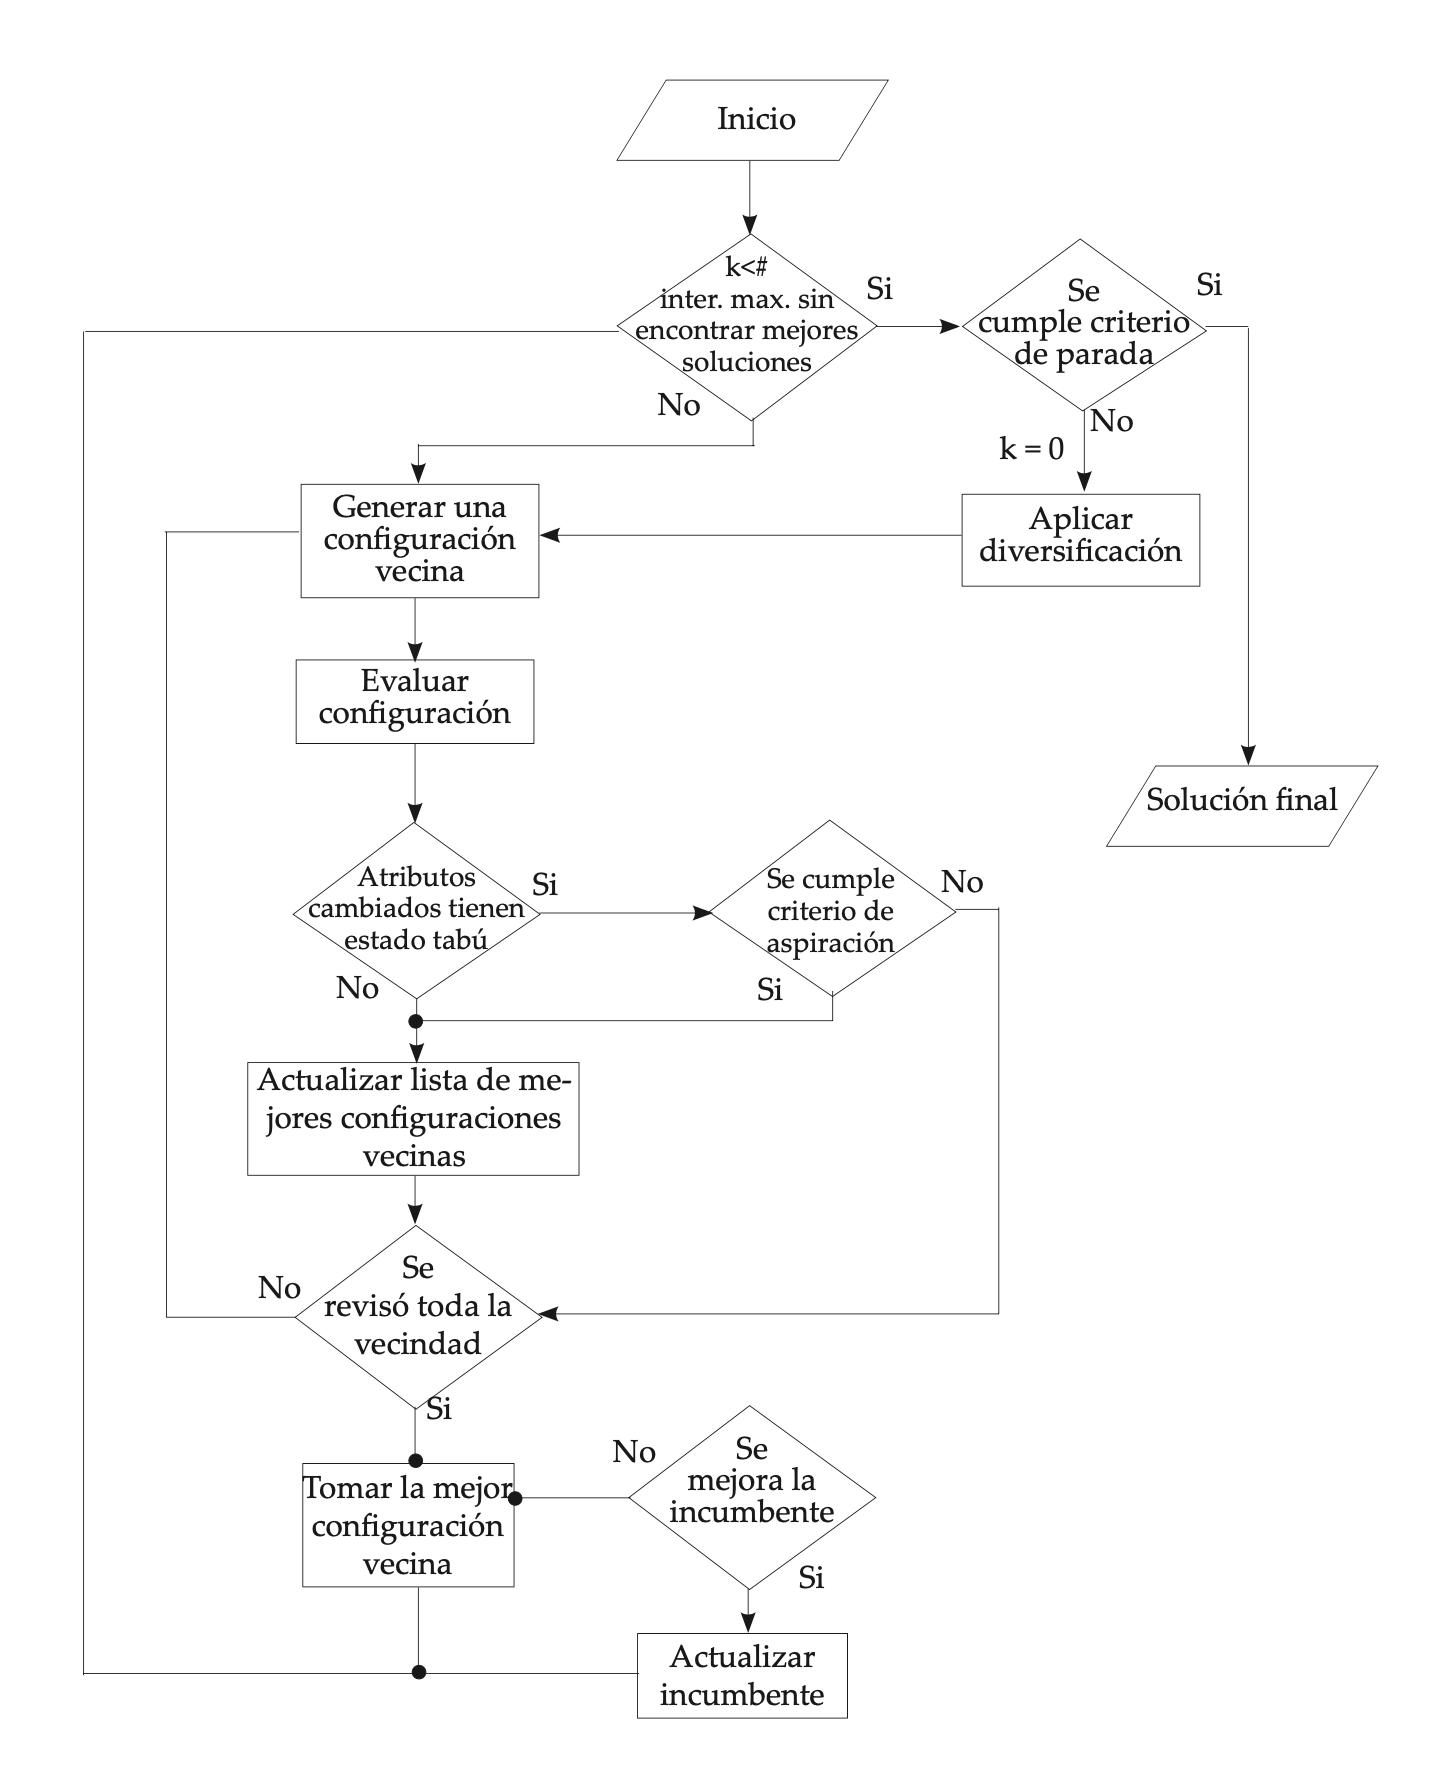
\includegraphics[scale=0.45]{assets/tabu.png}
\end{figure}
\section{Conclusiones}
El problema es \textit{complejo} por las variables relacionadas y condiciones involucradas.

Como la forma en la que se generan la configuaración inicial es \textit{eficiente} por lo que el número
de iteraciones necesarias en la estapa de la Búsqueda Tabú para las restricciones duras es menor porque desde
un principio se hacen movimientos que lo que buscan es evitar restricciones duras y que se reduzcan.

Los movimientos propuestos para generar vecindarios tienen la capacidad junto con las estrategias de
Búsqueda Tabú de escapar de ótimos locales y minimizar ambas restricciones. Esto se hace cuando el
proceso de búsqueda no mejora después de un número determinado de iteraciones.

Al final este artículo aborda este problema a su manera presentando la forma en como lo modelaron y
lo resolvieron.

%%%%%%%%%%%%%%%%%%%%%%%%%%%%%%%%%%%%%%%%%%%%%%%%%%%%%%%%%%%%%%%%%%%%%%%%%%%%%%%%%%%%%%%%%



%%%%%%%%%%%%%%%%%%%%%%%%%%%%%%%%%%%%%%%%%%%%%%%%%%%%%%%%%%%%%%%%%%%%%%%%%%%%%%%%%%%%%%%%%
\begin{thebibliography}{}

    \bibitem{}
    Fredy, John \& Franco, John \& Toro, Eliana \& Ocampo, Toro \& Alfonso, Ramón \& Rendón, Gallego. (2008).
    Problema de asignación óptima de salones resuelto con Búsqueda Tabú. 

\end{thebibliography}
%%%%%%%%%%%%%%%%%%%%%%%%%%%%%%%%%%%%%%%%%%%%%%%%%%%%%%%%%%%%%%%%%%%%%%%%%%%%%%%%%%%%%%%%%

\end{document}